\documentclass{article}
\usepackage[paperwidth=210mm,paperheight=297mm, top = 30mm, bottom = 30mm]{geometry}
%\usepackage[hangul]{kotex}
\usepackage{kotex}
\usepackage[utf8]{inputenc}
\usepackage{enumitem}
\usepackage{indentfirst}
\usepackage{graphicx, subcaption, tikz}
\usepackage{amsmath, amssymb, amsthm, amsfonts, bm}
\usepackage{listings}

\title{2020 Spring MAS365 Numerical Analysis HW6}
\author{20160650 채지석}
\date{\today}

\setlist{  
  listparindent=\parindent,
  %parsep=0pt,
}

\lstset{frame=tb,
  language=Python,
  aboveskip=3mm plus 2mm,
  belowskip=3mm plus 2mm minus 2mm,
  showstringspaces=false,
  columns=flexible,
  basicstyle={\small\ttfamily},
  numbers=none,
  %numberstyle=\tiny\color{gray},
  %keywordstyle=\color{blue},
  %commentstyle=\color{dkgreen},
  %stringstyle=\color{mauve},
  breaklines=true,
  breakatwhitespace=true,
  frame=single,
  tabsize=4
}

\newtheorem{prob}{Problem}

\newcommand{\set}[1]{\left\{ {#1} \right\}}
\newcommand{\vecx}{\boldsymbol{x}}
\newcommand{\mat}[1]{\boldsymbol{#1}}
\newcommand{\mata}{\boldsymbol{A}}
\newcommand{\matb}{\boldsymbol{B}}
\newcommand{\rr}{\mathbb{R}}
\newcommand{\nn}{\mathbb{N}}
\newcommand{\zz}{\mathbb{Z}}
\newcommand{\cc}{\mathbb{C}}
\newcommand{\qq}{\mathbb{Q}}
\newcommand{\norm}[1]{\left\lVert#1\right\rVert}
\newcommand{\card}[1]{\left\lvert#1\right\rvert}
\newcommand{\posdef}{\succ\mat{0}}
\newcommand{\psd}{\succeq\mat{0}}
\newcommand{\trace}{\text{trace}}
\newcommand{\comment}[1]{}
\newcommand{\problem}{\begin{prob}\end{prob}}
                    

\begin{document}

\section*{Computer Assignment}
The program which does the required is submitted via KLMS along with this document. It performs two tasks, as required in the assignment sheet.

Firstly the program performs the Power method. The implementation details are straightforward, being a direct translation of the equations presented in Exercise 6.14. As in Assignment 5, the stop condition is set to be when the relative error is less than $10^{-6}$. 

After that the program performs the Lanczos method. In a broad sense the code is again a direct translation of equations (6.5.3.1a) and (6.5.3.1b) in the textbook. The iteration shall stop when a small value of $\card{\gamma_i}$ is met, and this threshold is again set to be $10^{-6}$. Our goal is to compute the full tridiagonal matrix which is similar to $A_7$, but the iteration may stop early when the number of iterations has reached the dimension of the Krylov space $K(q, A_7)$ where $q$ is the initial vector. When $q = e_1$ as indicated in the assignment sheet, this dimension turns out to be $25$. This fact can be verifed by using the symbolic computation module \texttt{sympy} and the Python code included in the appendix. Anyhow, if the Lanczos iteration terminates early, this means that the tridiagonal matrix we desire is actually a block diagonal matrix of tridiagonal matrices, and we have to find a new initial vector to initiate the iteration in order to compute the next block. Such initial vector must be orthogonal to all $q_i$'s computed up to that point, so we take the strategy of running through the canonical basis vectors and taking the orthogonal complement of the projections onto $\operatorname{span}(q_i)$ until we find a nonzero orthogonal complement.  

Once we obtain all $\gamma_i$'s and $\delta_i$'s the rest is simple: we pass the computed tridiagonal matrix into the function \texttt{numpy.linalg.eig} provided by the \texttt{numpy} package in order to compute the eigenvalues.

The computed maximum eigenvalues are presented as outputs, as we see below. As a comparison we also show the maximum eigenvalue obtained by using the \texttt{numpy}-provided function \texttt{numpy.linalg.eig}.
\begin{center}
    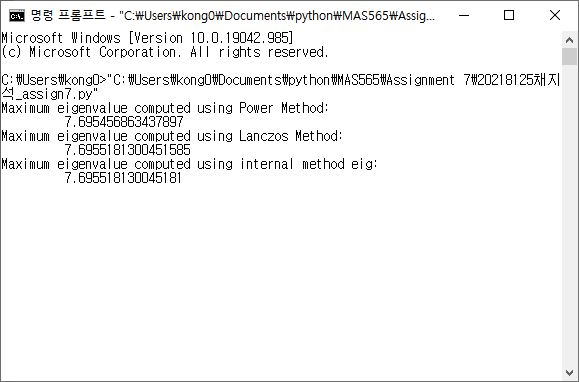
\includegraphics[width=0.75\linewidth]{console.JPG}
\end{center} Power method show a relative error of $7.96\times 10^{-6}$. However such seemingly large error is due to us setting the threshold to $10^{-6}$. If we set a smaller threshold we see that the Power method actually produces a result much closer to the result of \texttt{numpy.linalg.eig}. The performance of the Lanczos method is much more interesting. The result coinsides with the true value up to 14 digits. Again, we cannot conclude hastily that the result of the Lanczos method agrees with that of the Power method, since we allowed the Power method to stop early with low accuracy. If we increase the accuracy of the Power method, we see an agreement. 

It is also required to plot the eigenvalues of the computed tridiagonal matrix. The resulting plot is as the following figure. 
\begin{figure*}[th]
  \centering
  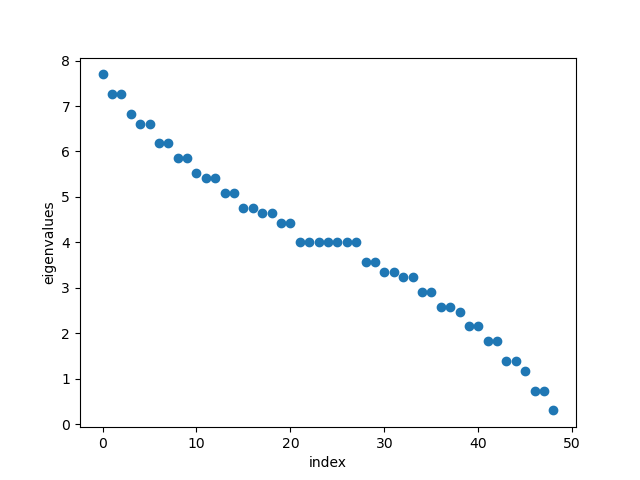
\includegraphics[width=0.75\textwidth]{3313.png}
  \caption{Scatter plot of the eigenvalues of $A_7$, in decreasing order}
  \label{fig:mean and std of net14}
\end{figure*}
  
\section*{Appendix}
The promised code, which computes the dimension of the Krylov space $K(e_1, A_7)$, is as follows. 

\begin{lstlisting}
  import numpy as np
  import sympy as sp
  
  def make_Tn(n):
      if n <= 0 :
          raise KeyError
      
      off_main_diag = [-1 for _ in range(n-1)]
      upper = np.diag(off_main_diag,  1)
      lower = np.diag(off_main_diag, -1)
      return 4*np.eye(n) + upper + lower
  
  def make_An(n):
      if n <= 0 :
          raise KeyError
  
      Tn = make_Tn(n)
      if n == 1 :
          return Tn
  
      I = np.eye(n)
      O = np.zeros((n,n))
  
      res = np.block([Tn, -I] + [O] * (n-2)) 
      for i in range(1, n-1):
          tmp = np.block([O] * (i-1) + [-I, Tn, -I] + [O] * (n-2-i))
          res = np.vstack((res, tmp))
      tmp = tmp = np.block([O] * (n-2) + [-I, Tn])
      res = np.vstack((res, tmp))
      return res
  
  n = 7
  A = sp.Matrix(np.array(make_An(n), dtype = int))
  e1 = sp.Matrix(np.array(np.hstack(([1], np.zeros(n**2-1))), dtype = int))
  
  K = e1
  for i in range(1, 49):
      e1 = A * e1
      K = K.col_insert(i, e1)
  
  print(K.rank())
  
  \end{lstlisting}
\end{document}